\chapter{Further Discuss on prediction method}
\label{ch:futuerDiscuss}


This chapter is about more test on the previous test conclusions. Here I just compare the top 3 method, that is Random Forest, Logistic Regression and SVM (As their training result is almost the same, here only test SVM) in stock direction prediction, Linear Regression, ANN and Random Forest in stock price accuracy test. All test are based on two years historical data. 

\section{Does Stock Price have effects on stock prediction results?}
\label{sec:priceInfluence}
To further discuss this topic, more test is needed. This section, stock tested number extend to 37 (All stock information can be found in Chapter~\ref{ch:stock_info}), the testing result is showed in figure~\ref{fg:furtherCDC} and \ref{fg:furtherMAPE}. 


\begin{figure}[h]
	\centering
	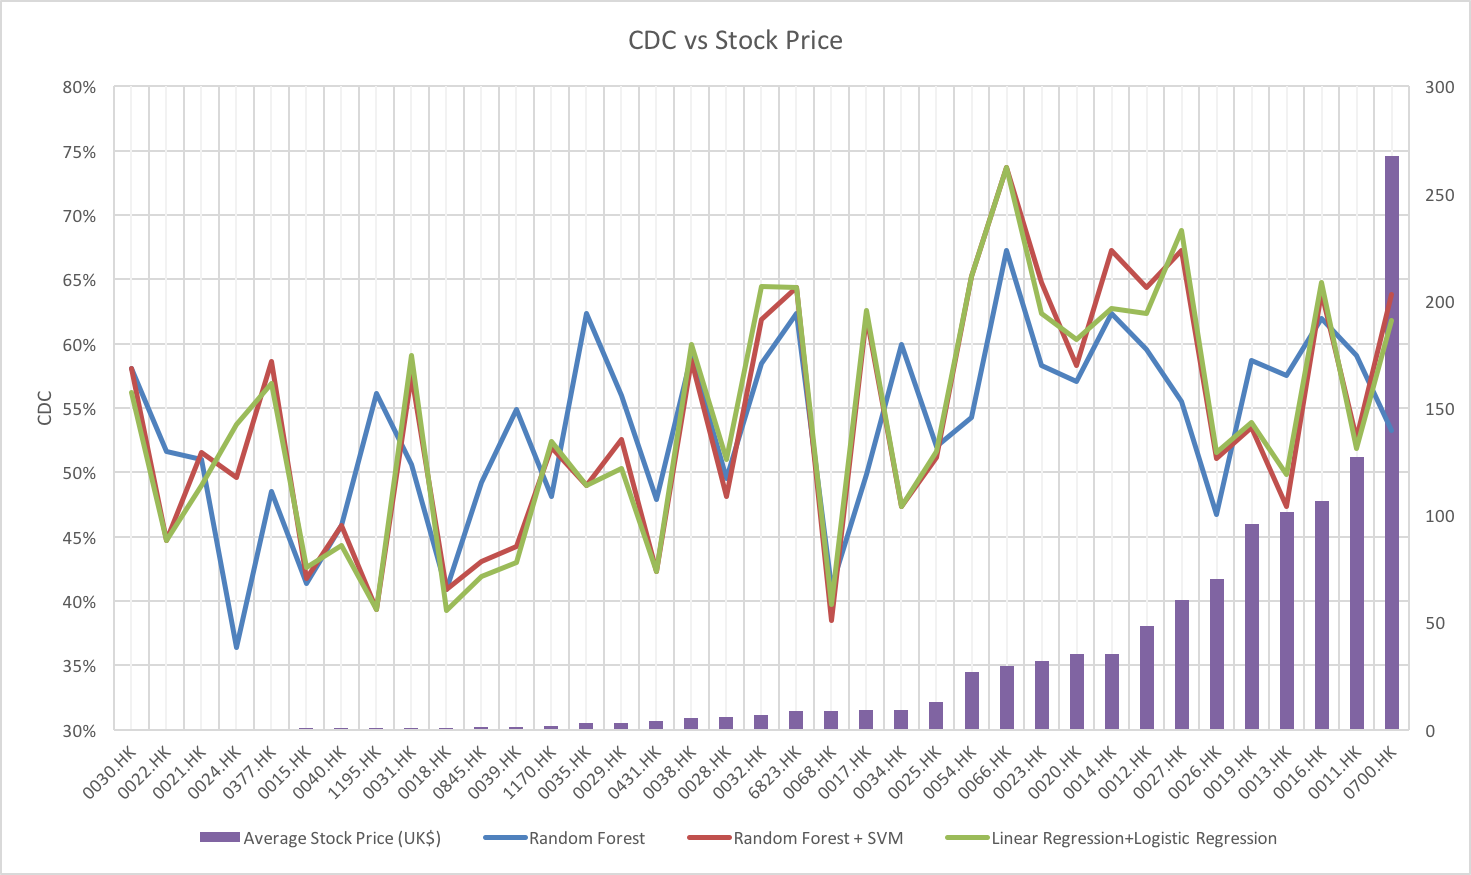
\includegraphics[width=0.8\textwidth]{FurtherDiscuss/CDCAVG}
	\caption{Extend result about stock price and CDC}
	\label{fg:furtherCDC}
\end{figure}


\begin{figure}[h]
	\centering
	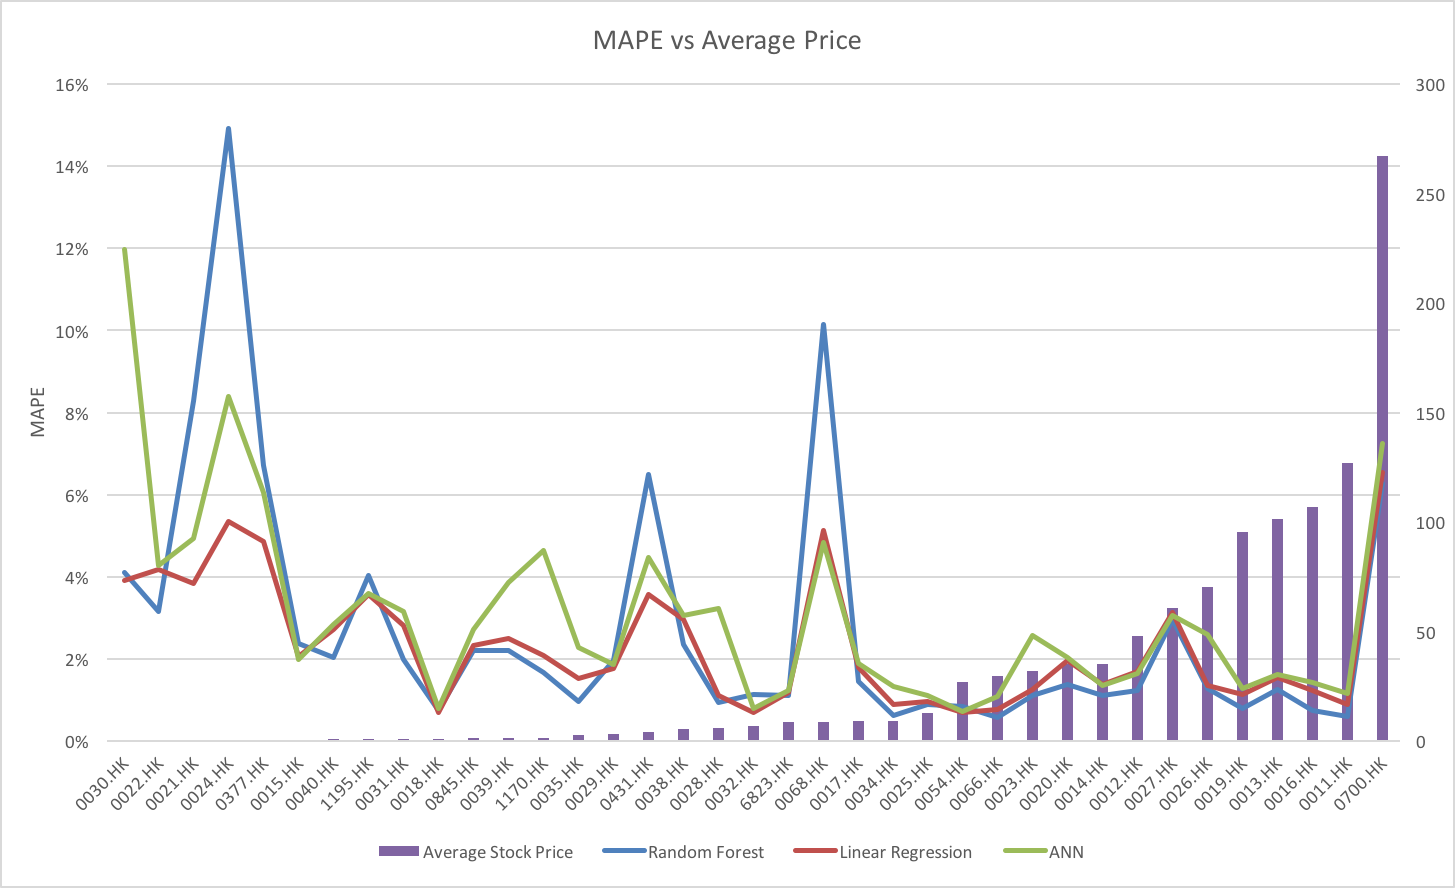
\includegraphics[width=0.8\textwidth]{FurtherDiscuss/MAPEAVG}
	\caption{Extend result about stock price and MAPE}
	\label{fg:furtherMAPE}
\end{figure}
\clearpage

The results show that stock price do not have relationship with the prediction result. It is true that MAPE of lower stock price seems to be larger than that of higher ones, this is because MAPE tends to have overestimate errors. For example, 0024.HK (Average stock price is \$0.3728 during the testing period), the MAPE of using Random Forest to predict its price is 14.92\%, its MAD is just 0.054, still a very small value.\\


All methods tends to reach its best performance at the same stock. For example, the CDC of 0066.HK, 6823.HK, 0014.HK, 0016.HK, 0012.HK, 0038.HK, 0032.HK, 0023.HK, 0030.HK, 0027.HK is above 60\% while using all method. This stock also performs well in its MAPE test. On the other hand, 0018.HK, 0068.HK, 0015.HK have a poor performance. Does it happens to be so? Or it is because the chosen input data is more suitable to predict those stock?


\section{Stock Performance on Specific Stocks with different time period}
This section is tried to answer the question, stock tested in this section is the stock with good and bad performance in section~\ref{sec:priceInfluence} add 0002.HK, which also have a good performance in Chapter~\ref{ch:AccuracyResult}.\\

\subsection{Test period 1 [from 2013-01-06 to 2016-01-06]}
The data slot is from 2013-01-06 to 2016-01-06 (former two years as training data and later 1 years as testing data, training dataset size is 472, testing is 247).

\begin{figure}[h]
	\centering
	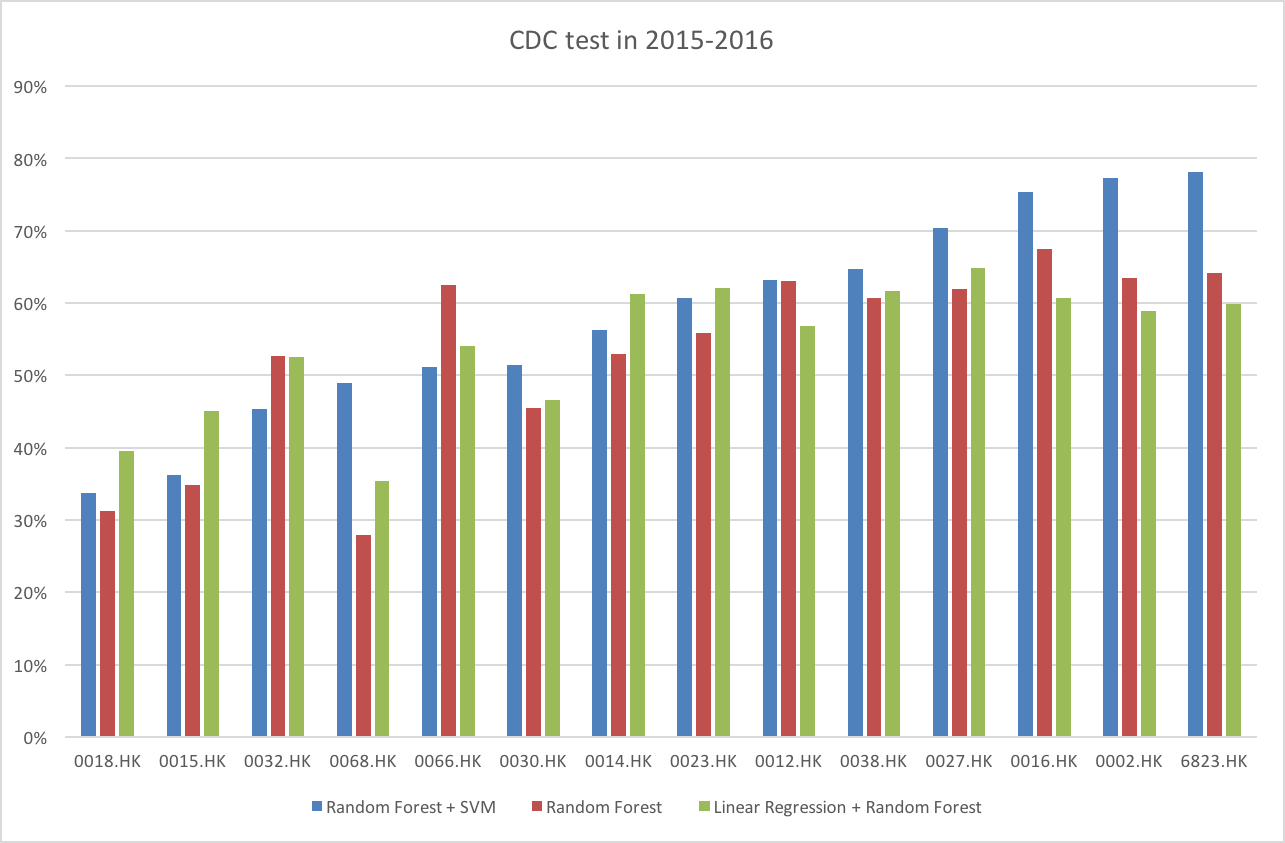
\includegraphics[width=0.8\textwidth]{FurtherDiscuss/CDC2016}
	\caption{Extend result about stock price and CDC}
	\label{fg:furtherCDC2016}
\end{figure}


\begin{figure}[h]
	\centering
	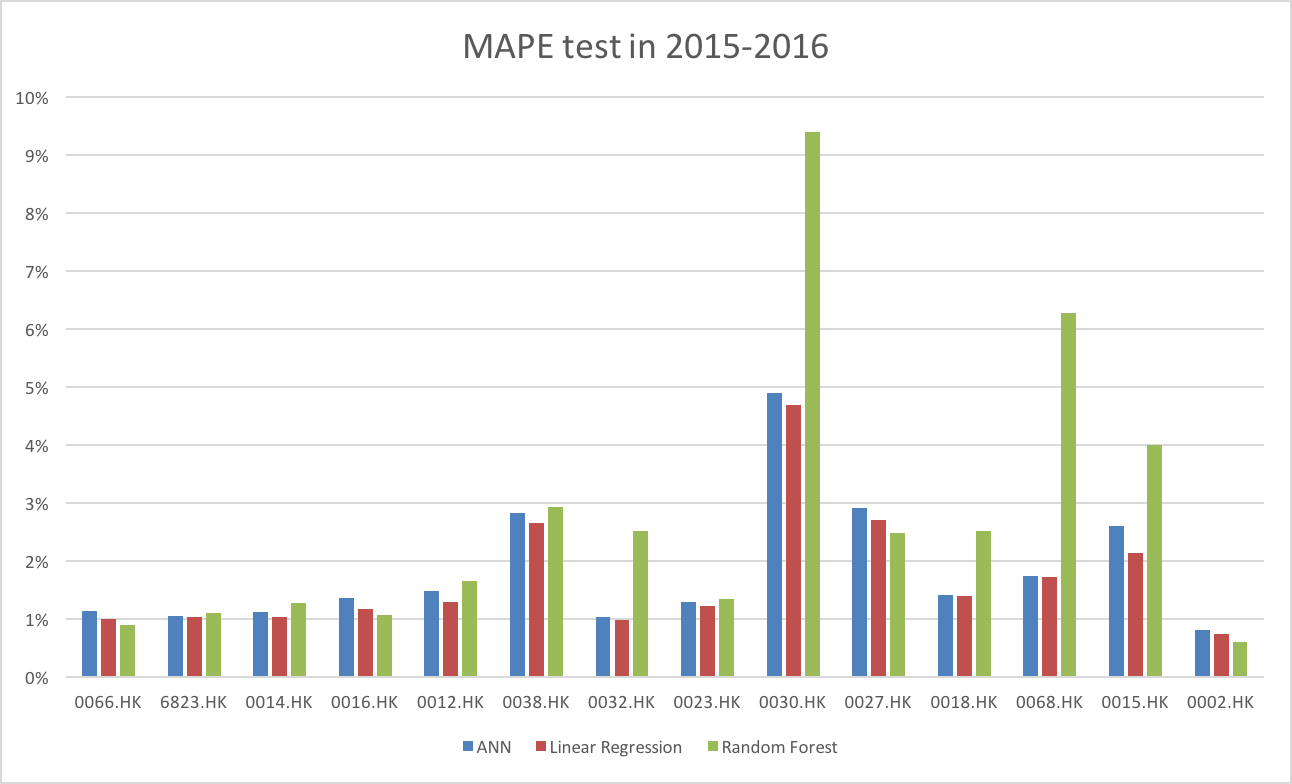
\includegraphics[width=0.8\textwidth]{FurtherDiscuss/MAPE2016}
	\caption{Extend result about stock price and MAPE}
	\label{fg:furtherMAPE2016}
\end{figure}
\clearpage
The performance trend still holds in CDC test (except for 0032.HK and 0030.HK). Other deductions also hold, Linear Regression and ANN are the best algorithm in predicting stock price changing amount, and SVM are the best method to predict stock change direction.

\subsection{Test period 2 [from 2009-01-06 to 2012-01-06]}
The data slot is from 2009-01-06 to 2012-01-06 (former two years as training data and later 1 years as testing data, training dataset size is 499, testing is 256).

\begin{figure}[h]
	\centering
	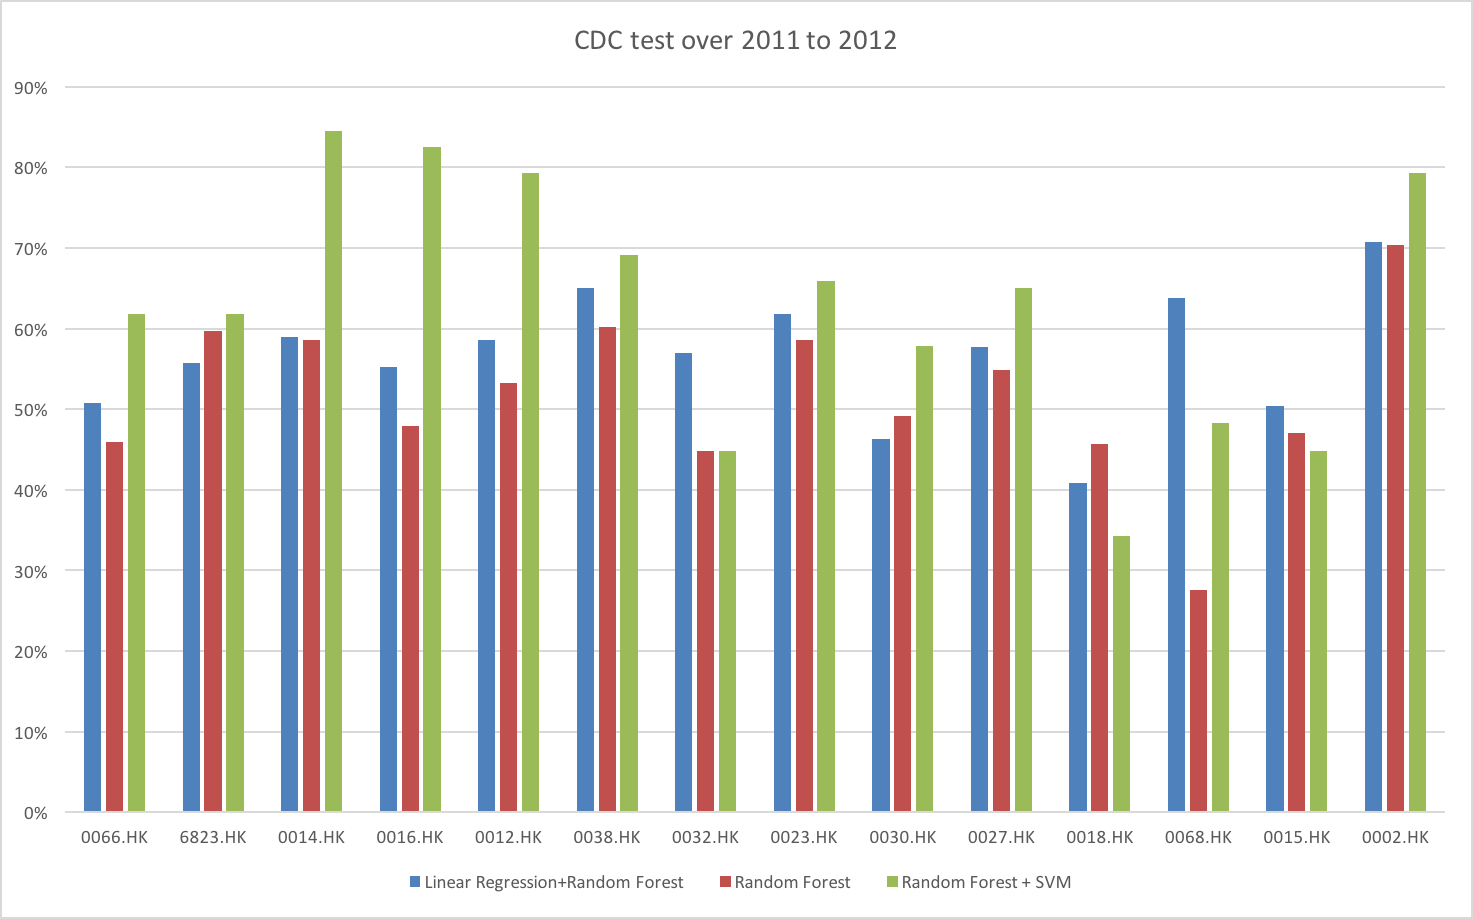
\includegraphics[width=0.8\textwidth]{FurtherDiscuss/CDC2012}
	\caption{Extend result about stock price and CDC}
	\label{fg:furtherCDC2012}
\end{figure}


\begin{figure}[h]
	\centering
	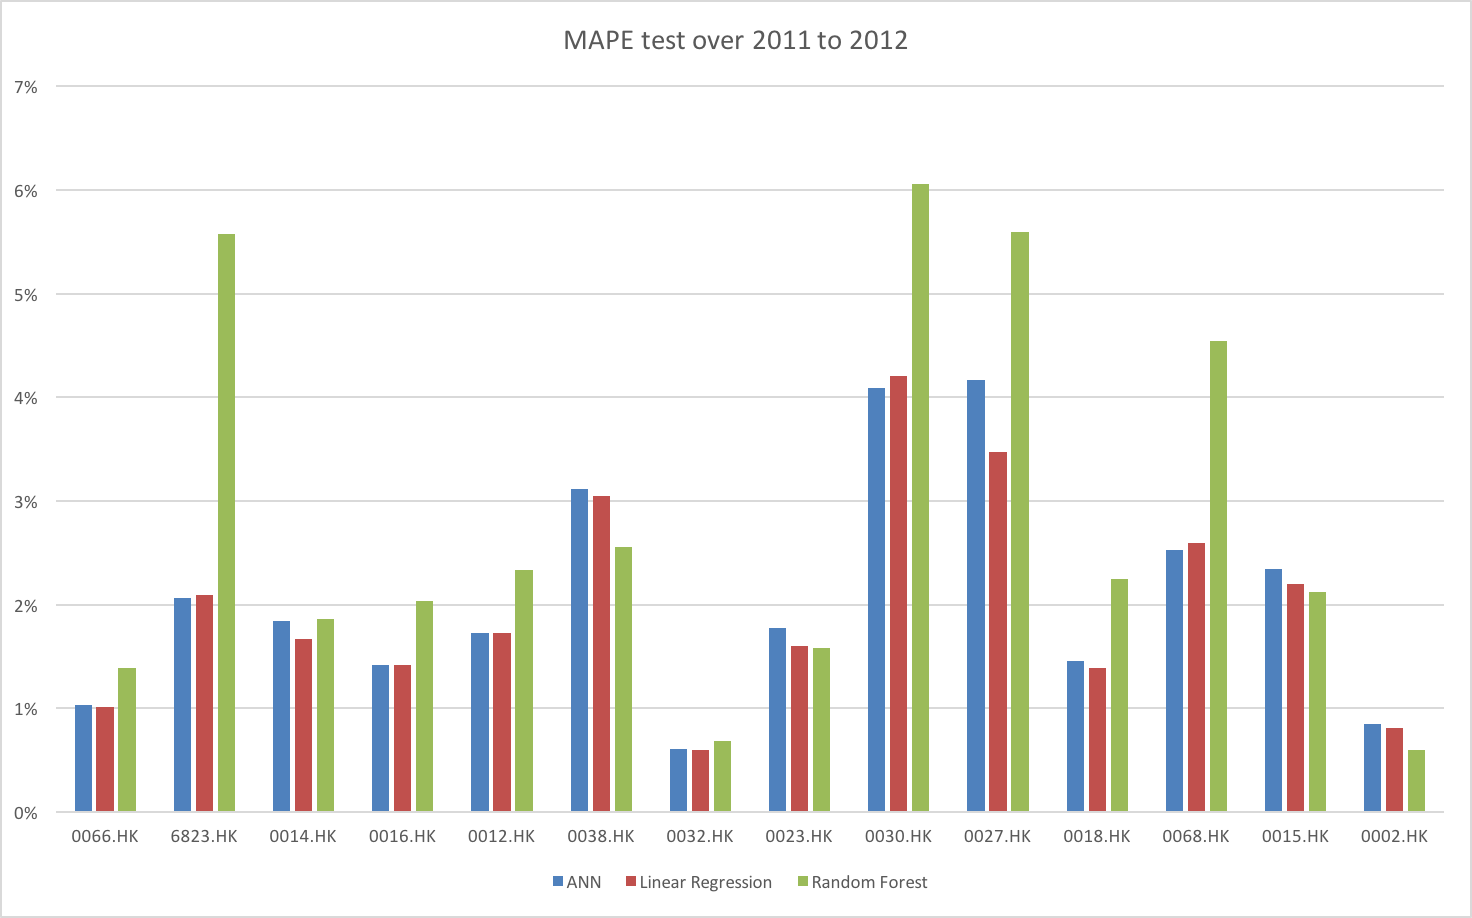
\includegraphics[width=0.8\textwidth]{FurtherDiscuss/MAPE2012}
	\caption{Extend result about stock price and MAPE}
	\label{fg:furtherMAPE2012}
\end{figure}

CDC test result can be found in figure\ref{fg:furtherCDC2012}. During this period, SVM is still the best method to forecast stock change direction, and except 0032.HK all the stocks keeps perform well in CDC test. And performance of 0018.HK, 0015.HK is still not very good. \\


For MAPE Test (result showed in figure~\ref{fg:furtherMAPE2012}), ANN and Linear Regression is the most reliable tools to predict stock price.

\subsection{Test period 3 [from 2010-01-06 to 2013-01-06]}
The data slot is from 2010-01-06 to 2013-01-06 (former two years as training data and later 1 years as testing data, training dataset size is 495, testing is 246).
\clearpage

\begin{figure}[h]
	\centering
	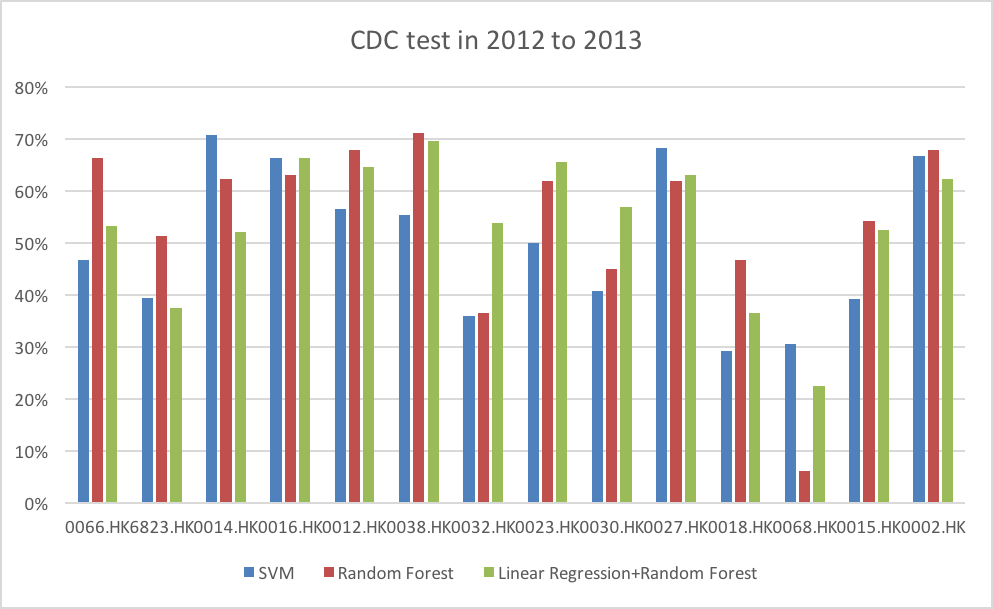
\includegraphics[width=0.8\textwidth]{FurtherDiscuss/CDC2013}
	\caption{Extend result about stock price and CDC}
	\label{fg:furtherCDC2013}
\end{figure}


\begin{figure}[h]
	\centering
	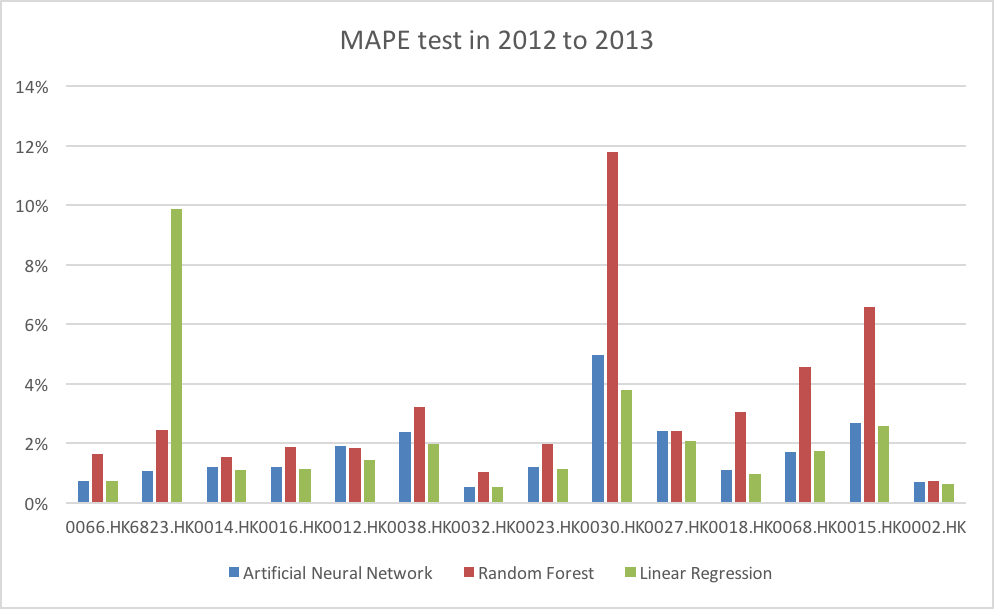
\includegraphics[width=0.8\textwidth]{FurtherDiscuss/MAPE2013}
	\caption{Extend result about stock price and MAPE}
	\label{fg:furtherMAPE2013}
\end{figure}

6823.HK drops greatly in CDC and MAPE, this is because of a great price gap between testing and training data. Its price was around HKD 0.5 before Dec 8, 2011, and went up to HKD 4.38 after Dec 9, 2011. That means the price of training data is only less than one of nine that of testing.\\


From the above test, another reason may holds for the performance. The active trading days (business day with stock transactions) during 2009-01-06 and 2015-01-06 are showed in figure~\ref{fg:activeTradingDays}. The reason for failing to predict the change direction is because lack of energy and the impact of suspension.


\begin{figure}[h]
	\centering
	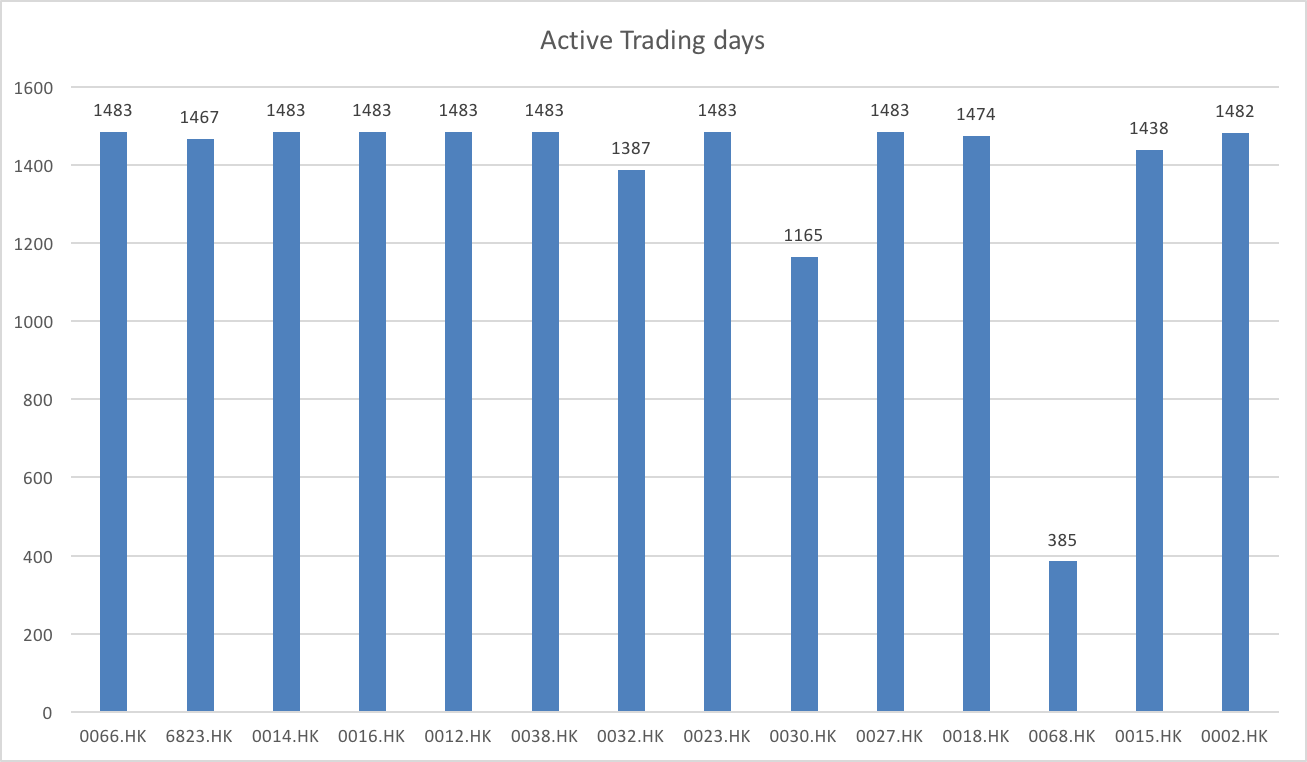
\includegraphics[width=0.8\textwidth]{FurtherDiscuss/activeTradeDays}
	\caption{Active trading days of every tested stock}
	\label{fg:activeTradingDays}
\end{figure}

\section{Testing on algorithm favor of a specific stock}
The above test show that our algorithm may have a favor over some type of stocks. '0902.HK' and '0836.HK' (which the same industry tag with '0002.HK', Utilities - Utilities - Electricity), '0315.HK'(Share the same industry with 6823.HK, Telecommunications - Telecommunications), '2282.HK' and '0120.HK' (share the same tag with '0027.HK', Consumer Services - Hotels, Casinos, Restaurants \& Leisure Facilities - Casinos \& Gaming). Test time is from 2012-01-06 to 2015-01-06.

\begin{figure}[h]
	\centering
	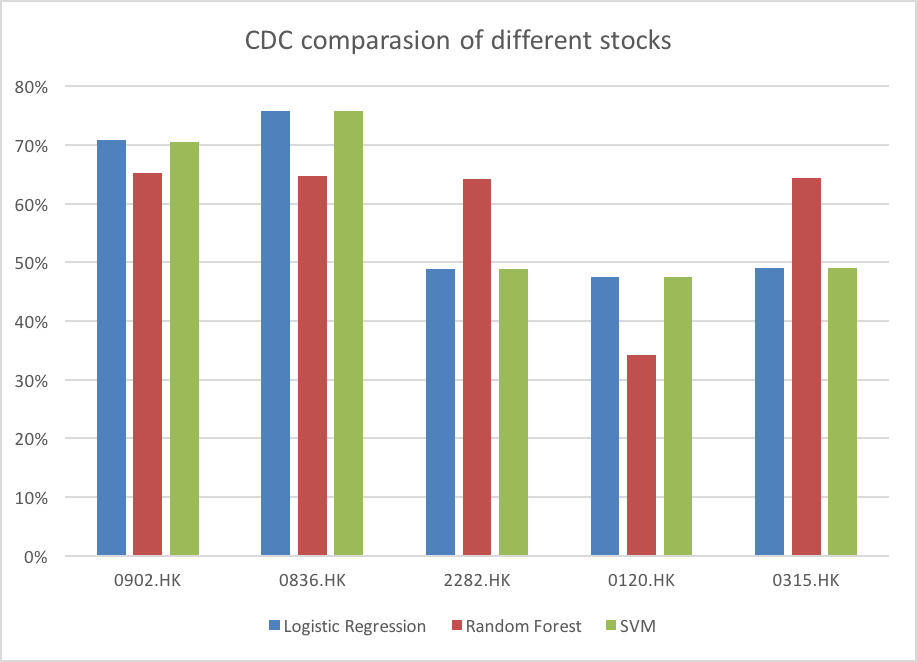
\includegraphics[width=0.8\textwidth]{FurtherDiscuss/CDCEXT}
	\caption{CDC test on other stock with same industries}
	\label{fg:furtherCDCEXT}
\end{figure}

\begin{figure}[t]
	\centering
	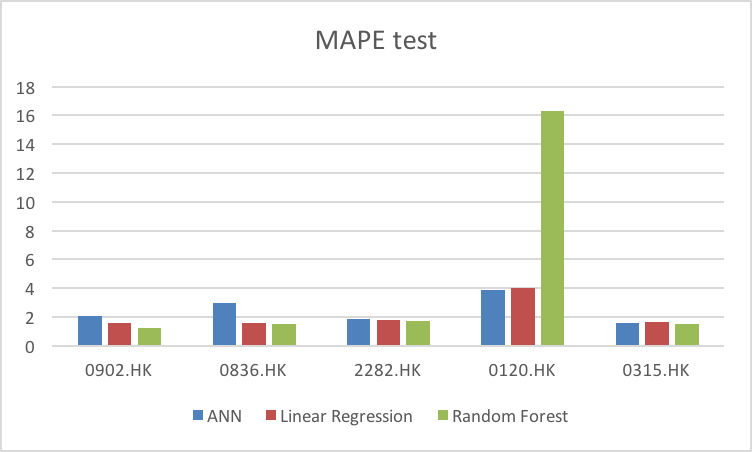
\includegraphics[width=0.8\textwidth]{FurtherDiscuss/MAPEEXT}
	\caption{MAPE test on other stock with same industries}
	\label{fg:furtherMAPEEXT}
\end{figure}


It seems that the input data have strong relationship with the stock price of Electricity industries, but not so for Consumer Services or Telecommunications. All stocks performs well in MAPE test (the average stock price of 0120.HK during testing period is HK\$0.11, the second smallest value is 0902.HK with HK\$8.39) is around 1.5\% error for every stocks, which is still reliable. Some learning methods struggle to handle this situation, e.g. the worsest MAPE of random forest is 131.52\%, linear regression also not performs well.